%\documentclass[handout,landscape]{beamer}
\documentclass[landscape]{beamer}
%\hypersetup{pdfpagemode=FullScreen}
\mode<handout>
{
  \usepackage{pgf}
  \usepackage{pgfpages}

\pgfpagesdeclarelayout{6 on 1 boxed}
{
  \edef\pgfpageoptionheight{\the\paperheight} 
  \edef\pgfpageoptionwidth{\the\paperwidth}
  \edef\pgfpageoptionborder{0pt}
}
{
  \pgfpagesphysicalpageoptions
  {%
    logical pages=6,%
    physical height=\pgfpageoptionheight,%
    physical width=\pgfpageoptionwidth%
  }
  \pgfpageslogicalpageoptions{1}
  {%
    border code=\pgfsetlinewidth{2pt}\pgfstroke,%
    border shrink=\pgfpageoptionborder,%
    resized width=.5\pgfphysicalwidth,%
    resized height=.5\pgfphysicalheight,%
    center=\pgfpoint{.25\pgfphysicalwidth}{.833\pgfphysicalheight}%
  }%
  \pgfpageslogicalpageoptions{2}
  {%
    border code=\pgfsetlinewidth{2pt}\pgfstroke,%
    border shrink=\pgfpageoptionborder,%
    resized width=.5\pgfphysicalwidth,%
    resized height=.5\pgfphysicalheight,%
    center=\pgfpoint{.75\pgfphysicalwidth}{.833\pgfphysicalheight}%
  }%
  \pgfpageslogicalpageoptions{3}
  {%
    border code=\pgfsetlinewidth{2pt}\pgfstroke,%
    border shrink=\pgfpageoptionborder,%
    resized width=.5\pgfphysicalwidth,%
    resized height=.5\pgfphysicalheight,%
    center=\pgfpoint{.25\pgfphysicalwidth}{.5\pgfphysicalheight}%
  }%
  \pgfpageslogicalpageoptions{4}
  {%
    border code=\pgfsetlinewidth{2pt}\pgfstroke,%
    border shrink=\pgfpageoptionborder,%
    resized width=.5\pgfphysicalwidth,%
    resized height=.5\pgfphysicalheight,%
    center=\pgfpoint{.75\pgfphysicalwidth}{.5\pgfphysicalheight}%
  }%
  \pgfpageslogicalpageoptions{5}
  {%
    border code=\pgfsetlinewidth{2pt}\pgfstroke,%
    border shrink=\pgfpageoptionborder,%
    resized width=.5\pgfphysicalwidth,%
    resized height=.5\pgfphysicalheight,%
    center=\pgfpoint{.25\pgfphysicalwidth}{.167\pgfphysicalheight}%
  }%
  \pgfpageslogicalpageoptions{6}
  {%
    border code=\pgfsetlinewidth{2pt}\pgfstroke,%
    border shrink=\pgfpageoptionborder,%
    resized width=.5\pgfphysicalwidth,%
    resized height=.5\pgfphysicalheight,%
    center=\pgfpoint{.75\pgfphysicalwidth}{.167\pgfphysicalheight}%
  }%
}


  \pgfpagesuselayout{6 on 1 boxed}[letterpaper, border shrink=5mm]
  \nofiles
}

\usepackage{listings}
%\lstset{language=TeX}
\usepackage{multimedia}
\usepackage[normalem]{ulem}
\usepackage{amssymb}

%\usecolortheme[named=Purple]{structure} 
%\usetheme{Copenhagen}
\usetheme{Warsaw} 
\usecolortheme{seahorse}
\useoutertheme{infolines} 
%\usetheme[height=7mm]{Rochester} 
%\setbeamertemplate{items}[ball] 
\setbeamertemplate{blocks}[rounded][shadow=true] 
%\setbeamertemplate{navigation symbols}{} 
\author{Joe Fields}
\title{Introduction to Proof} 
%\subtitle{}
\date{Lecture 8 (GIAM \S 2.1)}
\institute[SCSU]{ {\tt fieldsj1@southernct.edu} }

\newcommand{\versionNum}{$3.2$\ }

\newboolean{InTextBook}
\setboolean{InTextBook}{false}
\newboolean{InWorkBook}
\setboolean{InWorkBook}{false}
\newboolean{InHints}
\setboolean{InHints}{false}

%When this boolean is true (beginning in Section 5.1) we will use the convention
% that $0 \in \Naturals$.  If it is false we will continue to count $1$ as the smallest
%natural number (thus making Giuseppe Peano spin in his grave...)
 
\newboolean{ZeroInNaturals}

%This boolean is used to distinguish the version where we use $\sim$ rather than $\lnot$

\newboolean{LNotIsSim}

%The values of the last two booleans are set in ``switches.tex''

\setboolean{ZeroInNaturals}{true}
\setboolean{LNotIsSim}{false}


\let\savedlnot\lnot
\ifthenelse{\boolean{LNotIsSim}}{\renewcommand{\lnot}{\sim} }{}

%This command puts different amounts of space depending on whether we are
% in the text, the workbook or the hints & solutions manual. 
\newcommand{\twsvspace}[3]{%
 \ifthenelse{\boolean{InTextBook} }{\vspace{#1}}{%
  \ifthenelse{\boolean{InWorkBook} }{\vspace{#2}}{%
   \ifthenelse{\boolean{InHints} }{\vspace{#3}}{} %
   }%
  }%
 }


\newcommand{\wbvfill}{\ifthenelse{\boolean{InWorkBook}}{\vfill}{}}
\newcommand{\wbitemsep}{\ifthenelse{\boolean{InWorkBook} }{\rule[-24pt]{0pt}{60pt}}{}}
\newcommand{\textbookpagebreak}{\ifthenelse{\boolean{InTextBook}}{\newpage}{}}
\newcommand{\workbookpagebreak}{\ifthenelse{\boolean{InWorkBook}}{\newpage}{}}
\newcommand{\hintspagebreak}{\ifthenelse{\boolean{InHints}}{\newpage}{}}

\newcommand{\hint}[1]{\ifthenelse{\boolean{InHints}}{ {\par \hspace{12pt} \color[rgb]{0,0,1} #1 } }{}}
\newcommand{\inlinehint}[1]{\ifthenelse{\boolean{InHints}}{ { \color[rgb]{0,0,1} #1 } }{}}

\newlength{\cwidth}
\newcommand{\cents}{\settowidth{\cwidth}{c}%
\divide\cwidth by2
\advance\cwidth by-.1pt
c\kern-\cwidth
\vrule width .1pt depth.2ex height1.2ex
\kern\cwidth}

\newcommand{\sageprompt}{ {\tt sage$>$} }
\newcommand{\tab}{\rule{20pt}{0pt}}
\newcommand{\blnk}{\rule{1.5pt}{0pt}\rule{.4pt}{1.2pt}\rule{9pt}{.4pt}\rule{.4pt}{1.2pt}\rule{1.5pt}{0pt}}
\newcommand{\suchthat}{\; \rule[-3pt]{.5pt}{13pt} \;}
\newcommand{\divides}{\!\mid\!}
\newcommand{\tdiv}{\; \mbox{div} \;}
\newcommand{\restrict}[2]{#1 \,\rule[-4pt]{.25pt}{14pt}_{\,#2}}
\newcommand{\lcm}[2]{\mbox{lcm} (#1, #2)}
\renewcommand{\gcd}[2]{\mbox{gcd} (#1, #2)}
\newcommand{\Naturals}{{\mathbb N}}
\newcommand{\Integers}{{\mathbb Z}}
\newcommand{\Znoneg}{{\mathbb Z}^{\mbox{\tiny noneg}}}
\ifthenelse{\boolean{ZeroInNaturals}}{%
  \newcommand{\Zplus}{{\mathbb Z}^+} }{%
  \newcommand{\Zplus}{{\mathbb N}} }
\newcommand{\Enoneg}{{\mathbb E}^{\mbox{\tiny noneg}}}
\newcommand{\Qnoneg}{{\mathbb Q}^{\mbox{\tiny noneg}}}
\newcommand{\Rnoneg}{{\mathbb R}^{\mbox{\tiny noneg}}}
\newcommand{\Rationals}{{\mathbb Q}}
\newcommand{\Reals}{{\mathbb R}}
\newcommand{\Complexes}{{\mathbb C}}
%\newcommand{\F2}{{\mathbb F}_{2}}
\newcommand{\relQ}{\mbox{\textsf Q}}
\newcommand{\relR}{\mbox{\textsf R}}
\newcommand{\nrelR}{\mbox{\raisebox{1pt}{$\not$}\rule{1pt}{0pt}{\textsf R}}}
\newcommand{\relS}{\mbox{\textsf S}}
\newcommand{\relA}{\mbox{\textsf A}}
\newcommand{\Dom}[1]{\mbox{Dom}(#1)}
\newcommand{\Cod}[1]{\mbox{Cod}(#1)}
\newcommand{\Rng}[1]{\mbox{Rng}(#1)}

\DeclareMathOperator\caret{\raisebox{1ex}{$\scriptstyle\wedge$}}

\newtheorem*{defi}{Definition}
\newtheorem*{exer}{Exercise}
\newtheorem{thm}{Theorem}[section]
\newtheorem*{thm*}{Theorem}
\newtheorem{lem}[thm]{Lemma}
\newtheorem*{lem*}{Lemma}
\newtheorem{cor}{Corollary}
\newtheorem{conj}{Conjecture}

\renewenvironment{proof}%
{\begin{quote} \emph{Proof:} }%
{\rule{0pt}{0pt} \newline \rule{0pt}{15pt} \hfill Q.E.D. \end{quote}}


\newcommand{\vs}{\rule{0pt}{12pt}}

\AtBeginSection[]
{
 \begin{frame}{Table of Contents} 
  \tableofcontents[currentsection]
 \end{frame}
}

%%%% SAVE %%%%
%{ %magic to get a full screen image...
%\setbeamertemplate{navigation symbols}{}  % hide navigation buttons 
%\setbeamertemplate{background canvas}{\centerline{\includegraphics 
%	[height=\paperheight]{Cantor_4.jpeg}}}
%\begin{frame}[plain]
%\rule{0pt}{0pt}
%\end{frame} 
%} %end of magic


\begin{document}

\begin{frame}[plain]
  \titlepage
\end{frame}


\section{intro}

\begin{frame}{atomic concepts}
\begin{itemize}
\item the dictionary problem \pause
\item undefined terms \pause
\item points and lines and points on lines \pause (See Euclid) 
\end{itemize}
\end{frame}

\begin{frame}{postulates}
\begin{itemize}
\item Sentences involving the undefined terms that can't be proved. \pause
\item Euclid had 5 ``postulates'' and 5 ``common notions.'' \pause
\item Axioms
\end{itemize}
\end{frame}

\begin{frame}{atomic concepts in logic}
\begin{itemize}
\item True and False 
\item Sentences
\end{itemize}
\end{frame}

\begin{frame}{statements}
\begin{itemize}
\item A sentence that is either True or False.\pause
\item Ambiguity \pause
\item Undecideability 
\end{itemize}
\end{frame}

\section{connectors}

\begin{frame}{compound statements}
\begin{itemize}
\item And and but. \pause
\item ``They turned off my electricity, but I paid the bill!'' \pause
\item Or \pause
\item ``Close the door or bugs will get in the house.'' \pause
\item Conjunction and Disjunction
\end{itemize}
\end{frame}

\begin{frame}{predicate variables}
\begin{itemize}
\item We can use variables to stand for entire sentences. \pause
\item Example $P =$ ``The electricity has been shut off.'' and $Q =$ ``The electric bill was paid.'' \pause
\item We use the symbols $\land$ and $\lor$ to hook predicates together to make more complicated {\em compound sentences}. \pause
\item $\land$ -- conjunction -- and \pause
\item $\lor$ -- disjunction -- or \pause
\item $P \land Q$ is the same as ``They turned off my electricity, but I paid the bill!''
\end{itemize}
\end{frame}

\begin{frame}{truth tables}
\begin{itemize}
\item There are four possibilities for the truth or falsity of a pair of unrelated statements.\pause
\item We use the symbols $T$ and $\phi$ for true and false (respectively). \pause
\end{itemize}

\begin{center}
\begin{tabular}{c|c}
The sun is shining \; & \; It is raining \\ \hline
T & T \\
T & $\phi$ \\
 $\phi$ & T \\
 $\phi$ &  $\phi$ \\
\end{tabular}
\end{center}

\end{frame}

\begin{frame}{using truth tables}
\begin{itemize}
\item conjunction \pause
\item disjunction \pause
\item negation
\end{itemize}
\end{frame}

\section{a new kind of algebra}

\begin{frame}{Boolean algebra}
\begin{itemize}
\item Precedence of operators in ordinary algebra. \pause PEMDAS \pause
\item Multiplication is repeated addition. \pause
\item Exponentiation is repeated multiplication. \pause
\item The logical connectors $\land$ and $\lor$ don't have a predefined precedence. \pause
\item Logical negation ($\lnot$) binds more tightly than the others. \pause
\item Takeaway: use parentheses to ensure you communicate what you really mean.\pause
\item $A \land B \lor C$ ???
\end{itemize}
\end{frame}

\begin{frame}{digital logic circuits}
\begin{itemize}
\item Series connections implement AND. \pause
\item Parallel connections implement OR. \pause
\item The non-exclusive or. \pause
\end{itemize}

\begin{center}
\begin{picture}(0,0)%
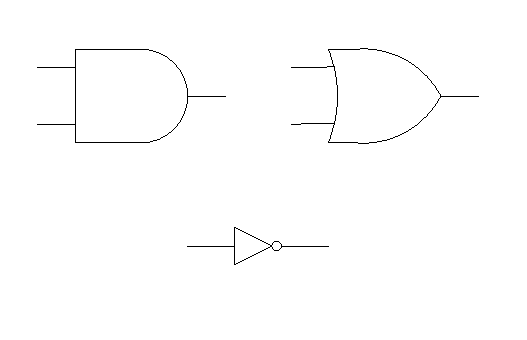
\includegraphics{figures/gates.pdf}%
\end{picture}%
\setlength{\unitlength}{3947sp}%
%
\begingroup\makeatletter\ifx\SetFigFont\undefined%
\gdef\SetFigFont#1#2#3#4#5{%
  \reset@font\fontsize{#1}{#2pt}%
  \fontfamily{#3}\fontseries{#4}\fontshape{#5}%
  \selectfont}%
\fi\endgroup%
\begin{picture}(4202,2702)(300,-2162)
\put(2026,-1861){\makebox(0,0)[lb]{\smash{{\SetFigFont{12}{14.4}{\familydefault}{\mddefault}{\updefault}{\color[rgb]{0,0,0}Not ($\lnot$)}%
}}}}
\put(2926,-961){\makebox(0,0)[lb]{\smash{{\SetFigFont{12}{14.4}{\familydefault}{\mddefault}{\updefault}{\color[rgb]{0,0,0}Or ($\lor$)}%
}}}}
\put(901,-961){\makebox(0,0)[lb]{\smash{{\SetFigFont{12}{14.4}{\familydefault}{\mddefault}{\updefault}{\color[rgb]{0,0,0}And ($\land$)}%
}}}}
\end{picture}%

\end{center}
\end{frame}

\begin{frame}{Understanding laws via logic circuits}
\begin{itemize}
\item Commutative law 
\item Associative law -- leads to a shorthand with multiple input gates \pause
\item Distributive law
\end{itemize}
\end{frame}

\begin{frame}{Getting a specified output}
\begin{itemize}
\item Recognizers \pause
\item Disjunctive normal form \pause (the OR of a bunch of ANDs) \pause
\item Figure 2.5 in GIAM
\end{itemize}
\end{frame}



\end{document}
